\documentclass[a4paper, dutch, abstract=true]{scrartcl}
\usepackage[utf8]{inputenc}
\usepackage[dutch]{babel}
\usepackage{eurosym}
\usepackage{graphicx}
\graphicspath{{./afbeeldingen/}}
\usepackage[automark]{scrlayer-scrpage}
\usepackage[style=ieee]{biblatex}
\addbibresource{raspberry-pi.bib}
\title{Vergelijking het Raspberry Pi- en Arduinoplatform}
\subtitle{Papergroep 34}
\subject{INFONW Paper}
\author{
    Wilmar Duvekot\thanks{6523617} \and Luuk Berkers\thanks{6793592} \and Jacob-Jan Mosselman
    \thanks{6675522} \and Kenneth Man\thanks{6007767} \and Herman Horneman\thanks{6897630}
}
\date{28 oktober 2019}
\addtokomafont{pagehead}{\upshape}

\begin{document}
\maketitle

\begin{abstract}
    Dit onderzoek probeert een antwoord te geven op de vraag of een Arduino of een Raspberry Pi een
    betere mini-computer is.
    Het onderzoek geeft daarop een antwoord en ook op de vraag wat de verschillen precies zijn.
    De Arduino is een mini-computer die vooral handig kan zijn bij het automatiseren van processen,
    en de Raspberry Pi is een iets uitgebreidere computer met wat meer aansluitingen beschikbaar.
    Het grootste verschil is dat de Raspberry Pi een grotere processor heeft dan de Arduino.
    Hieruit wordt geconcludeerd dat de Raspberry Pi het beste gebruikt kan worden voor grote
    opdrachten en dat de Arduino geschikt is voor kleinere, simpele opdrachten.
\end{abstract}

\tableofcontents

\section{Inleiding}
In de laatste decennia heeft technologie een enorme ontwikkeling doorgemaakt.
Zo zijn de telefoons uitgevonden en zijn deze steeds kleiner, sneller en beter geworden.
Televisie heeft kleur gekregen en er zijn steeds meer zenders te zien.
Ook heeft de computer een enorme ontwikkeling doorgemaakt.
De computers van vroeger konden klaslokalen vullen, maar tegenwoordig kunnen ze in een rugzak
meegenomen worden.
De laptop wordt steeds kleiner, steeds sneller en gaat ook steeds beter presteren.
De technologie gaat tegenwoordig zelfs zo ver, dat een fotolijstje digitaal gemaakt kan worden,
zodat mensen foto's naar het lijstje kunnen sturen en dat het lijstje die foto's dan laat zien, een
voorbeeld daarvan is de Claudia digitale fotolijst \cite{innovu2019fotolijst}.

De technologie wordt steeds kleiner en beter dus, dat is ook te zien aan de mini-computers.
De Raspberry Pi \cite{raspberry2019raspberry} en de Arduino \cite{arduino2019arduino} zijn ongeveer
even groot als een telefoon en ze kunnen veel.
Het principe is hetzelfde als een laptop of computer
De computers kunnen worden geprogrammeerd, en ze kunnen in principe alles doen, zolang het
geprogrammeerd wordt.
De Arduino en Raspberry Pi zullen in dit onderzoek verder uitgelegd worden.

Dit onderzoek zal gaan over de verschillen tussen de Arduino en Raspberry Pi, zodat duidelijk wordt
wat met de mini-computers gedaan kan worden en wat het nut kan zijn in de samenleving.
De onderzoeksvraag luidt: Wat zijn de verschillen tussen Raspberry Pi en Arduino en welke is beter?
Op deze vraag zal een antwoord gevonden worden in dit paper.
Dit paper zal beginnen met informatie over de Arduino, de architectuur, hardware, software en
toepassingen.
Vervolgens zal er worden verteld over de Raspberry Pi, architectuur, hardware, software en
toepassingen.
Daarna zullen verschillen en overeenkomsten besproken worden.
Vervolgens volgt de conclusie en de appendix.

\section{Arduino}
Dit paper zal beginnen met te vertellen hoe een Arduino in elkaar zit.
Dit zal gebeuren aan de hand van de architectuur en de hardware van de Arduino.
Vervolgens wordt er gekeken naar de software van de Arduino en er wordt als laatst gekeken naar de
toepassingen en mogelijkheden.

\subsection{Architectuur \& Hardware}
De Arduino is een singleboardcomputer en bestaat uit de basis van alle componenten waar een
hedendaagse computer ook uit bestaat, zoals een processor, RAM en I/O.
De meeste Arduinos hebben een singlecoreprocessor maar er zijn ook wel multicore Arduinos
verkrijgbaar.
Deze Arduinos met multicoreprocessors zijn vooral nuttig voor het parallel uitvoeren van
verschillende taken.
De hoeveelheid RAM verschilt per Arduino en loopt van minimaal 8 kB tot maximaal 32 kB aan RAM
\cite{arduino2019products}.
Dit is lang niet vergelijkbaar met het de hoeveelheid RAM in moderne pc's en laptops.
Dat is namelijk vele malen meer, maar voor een Arduino niet nodig gezien het doel waarmee de Arduino
geproduceerd wordt.

In het RAM worden processen ingeladen die uitgevoerd moeten gaan worden, maar er kan geen I/O data
permanent worden opgeslagen. 
Om toch I/O data permanent op te slaan wordt een SD kaartje gebruikt.  
De Arduino heeft ook de mogelijkheid om gekoppeld te worden aan een computer, waarbij de gegevens
van de Arduino op de harde schijf van de desbetreffende computer gezet kunnen worden.
In de nieuwere Arduinos kan wel data permanent worden opgeslagen. Daar wordt EEPROM voor gebruikt.
Er is ook flash memory aanwezig op de Arduino, deze wordt gebruikt om de programmas op te slaan 
zonder dat deze verloren gaan bij het opnieuw opstarten van de Arduino.
In tegenstelling tot RAM, waar alle data gewist wordt bij het herstarten.
Verder heeft de Arduino geen videokaart aangesloten zitten en kan niet gebruikt worden om data te visualiseren op een beeldscherm.
Daar is de Arduino dan ook niet voor bedoeld.

Hiernaast heeft de Arduino meerdere input/output pins.
Op de inputs worden sensoren aangesloten die verschillende waardes meten en deze aan de Arduino
meegeven.
Op de output wordt een actor aangesloten die met bepaalde berekeningen of uitkomsten uit de Arduino
een actie uitvoert.
Tussen de input en de output berekent de geschreven software iets met de data verkregen uit de input
en stuurt ook de actor aan \cite{arduinoreference}.

De hardware is open source, dat betekent dat willekeurige producenten het recht hebben om Arduino te
produceren en te verkopen.
Alleen de naam Arduino mag niet zonder meer gebruikt worden.

De Arduino is standaard voorzien van een bootloader \cite{optiboot2019github}, dit vergemakkelijkt
het proces om code werkend op de Arduino te krijgen.
Bij het starten van de Arduino wordt de bootloader gestart en deze wacht op de aangesloten computer
om een nieuw stuk software te ontvangen.
% ? Welk geheugen wordt hier bedoeld?
Zodra er nieuwe software wordt ontvangen zal deze worden weggeschreven in het geheugen van de
Arduino zodat deze later opnieuw kan worden uitgevoerd zonder dat de hoofdcomputer aangesloten hoeft
te zijn aan de Arduino.

\subsection{Software}
Zoals al gezegd zijn de meeste arduinoborden uitgerust met een singlecoreprocessor.
De Arduino is bedoeld om simpele programma's te laten runnen om een elektronicaproject aan te
sturen.
Hiervoor is meestal een singlecoreprocessor genoeg.
Wanneer de projecten echter groter worden, dan kan het handig zijn om verschillende taken parallel
uit te gaan voeren, zolang die taken maar niet achtereenvolgens uitgevoerd moeten worden kan dat
heel goed.
Het voordeel hiervan is dat dezelfde taken in een kortere periode uitgevoerd kunnen worden.
Om deze processen parallel uit te voeren is er een multicore processor nodig.

Zoals gezegd is heeft de Arduino erg weinig RAM vergeleken met moderne pc's, het is ook niet nodig
om meer RAM te hebben voor een Arduino omdat deze er op gebouwd is om kleine elektronicaprojecten
aan te sturen.
Hij doet dus kleine berekeningen en opdrachten en hoeft geen zware taken uit te voeren zoals het
aansturen van een beeldscherm.
Dit kan ook niet, onder andere omdat de Arduino geen videokaart heeft en hij is er ook niet voor
bedoeld om data op een beeldscherm te visualiseren.

De software programmeert men op een laptop of pc en laad je via een USB-kabel op de Arduino.
Het programmeren gebeurt met behulp van de Arduino IDE.
IDE staat voor Integrated Development Environment en is een volledige programmeeromgeving.
Arduino heeft zijn eigen programmeertaal ontwikkeld, deze is gebaseerd op C en C++.
De IDE van Arduino is ook open source \cite{arduino2019github}, dus men kan eigen aanpassingen
doorvoeren in het programma.

Je kan ook ISP gebruiken om je software op je Arduino te zetten.
ISP staat voor in-system programming.
Dit houd in dat de chip op de Arduino blijft zitten en alle componenten aangesloten blijven.
Waarna vervolgens de chip wordt geprogrammeerd door een andere Arduino.

\subsection{Mogelijkheden \& Toepassingen}
Zoals al eerder gezegd is de Arduino echt bedoeld om elektronicaprojecten aan te sturen.
Gegevens van de buitenwereld door middel van sensoren meten, waardes berekenen en vervolgens andere
hardware aansturen aan de hand van die waardes.

Er zijn tal van mogelijkheden met de Arduino, zo wordt hij vaak gebruikt om een smart home te
realiseren.
Lampen, wekkers, rookmelders, gordijnen, deuren etc. etc. worden aangesloten op een Arduino en vanaf
daar bestuurd.
Zo kan je de Arduino verbinden aan je netwerk en switches omzetten vanaf je telefoon.

Ook wordt de Arduino gebruikt om bepaalde processen te automatiseren, bijvoorbeeld het voeren van
katten.
Heel simpel kan de Arduino eens om de zoveel tijd eten in een bakje bijvullen.
Ook kan met een sensor eerst nog even gecheckt worden of er nog eten in zit.
Zo ja, dan hoeft het eten niet bijgevuld te worden.

Er kunnen ook camera's op een Arduino worden aangesloten.
Men kan bijvoorbeeld een Arduino monteren op een bestuurbare auto en door het juiste programmeerwerk
uit te voeren kan men de auto autonoom maken.
Dit is echter wel een project voor gevorderden aangezien hier kunstmatige intelligentie bij komt
kijken.
Men kan echter ook zelf de auto besturen en de arduino{\"o}bjecten laten herkennen.
Zo kan een seintje gegeven worden als een bepaald object gespot wordt.

Een andere toepassing is het beveiligen van objecten met behulp van een vingerafdrukscanner.
De input is een vingerafdruk.
Als de Arduino de vingerafdruk kan matchen met een vingerafdruk in een database die in het systeem
staat, wordt toegang verleend.
Zo kan een deur van het slot opengaan, een garagedeur automatisch openen, toegang geven tot kastjes
en/of diepvriezen.

Met een Arduino kan men ook lasersnijden.
Men geeft aan de Arduino mee welke vormen er gesneden moeten worden en de Arduino loopt keurig die
vorm af en snijdt zo het gewenste stuk uit een plaatje van een bepaald materiaal.

\paragraph*{}
Er is nu bekend wat de Arduino kan en hoe deze werkt
Om de onderzoeksvraag volledig te kunnen beantwoorden is het goed om zowel over de Arduino als over
de Raspberry Pi informatie te hebben.
Het volgende stuk in dit paper zal gaan over de Raspberry Pi en hoe deze werkt.

\section{Raspberry Pi}
Zoals in het vorige stuk genoemd, is het nodig om de mogelijkheden van de Raspberry Pi te
begrijpen om de onderzoeksvraag goed te beantwoorden.
Dit zal gaan op dezelfde manier als de Arduino ook is uitgelegd.
Eerst zal worden gekeken naar de architectuur en hardware.
Vervolgens naar de software van een Raspberry Pi en op het eind zullen toepassingen en mogelijkheden
besproken worden.

\subsection{Architectuur \& Hardware}
De Raspberry Pi is een volwaardige computer met een compact formaat.
Hij bevat dezelfde componenten die een volledige desktop-pc ook bevat, met als voordeel dat hij in
een broekzak past.
Bijkomend nadeel is wel dat men een aparte monitor, muis en toetsenbord moet aanschaffen als men de
Raspberry Pi als traditionele desktop computer wilt gebruiken.

In tegenstelling tot traditionele desktop pc's en laptops van de laatste 10 jaar is de Raspberry Pi
niet voorzien van een x86 processor.
De Raspberry Pi is voorzien van een ARM processor \cite{jain2014raspberry}.
Er bestaan op het moment van schrijven verschillen versies.
De Raspberry Pi 1 en Zero hebben een 32-bits architectuur, terwijl de Raspberry Pi's 2, 3 en 4 een
64-bits architectuur hebben.
Verder is de architectuur min of meer hetzelfde.
Alle Raspberry Pi's draaien op basis van een ARM processor.

Omdat er verschillende versies bestaan van de Raspberry Pi, wordt in dit paper de nadruk gelegd op
de Raspberry Pi 4.
Deze heeft een kloksnelheid van 1.5 GHz en een RAM van 1, 2 of 4 GB.
Afhankelijk van het Raspberry Pi 4 model dat men gekocht heeft, zal het RAM geheugen verschillend
zijn.
Kloksnelheid is wel voor alle modellen van de Raspberry Pi 4 hetzelfde.
Verder heeft hij in totaal vier USB poorten.
Namelijk twee USB 2.0 en 2 USB 3.0 poorten.
Ook heeft de Raspberry Pi 4 een Ethernet aansluiting waarmee een internetverbinding mogelijk is,
maar ook een directe verbinding met een andere computer \cite{maksimovic2014raspberry}.
Voor een internetverbinding beschikt de Raspberry Pi ook over wifi functionaliteit.

\subsection{Software}
\begin{figure}[h]
    \centering
    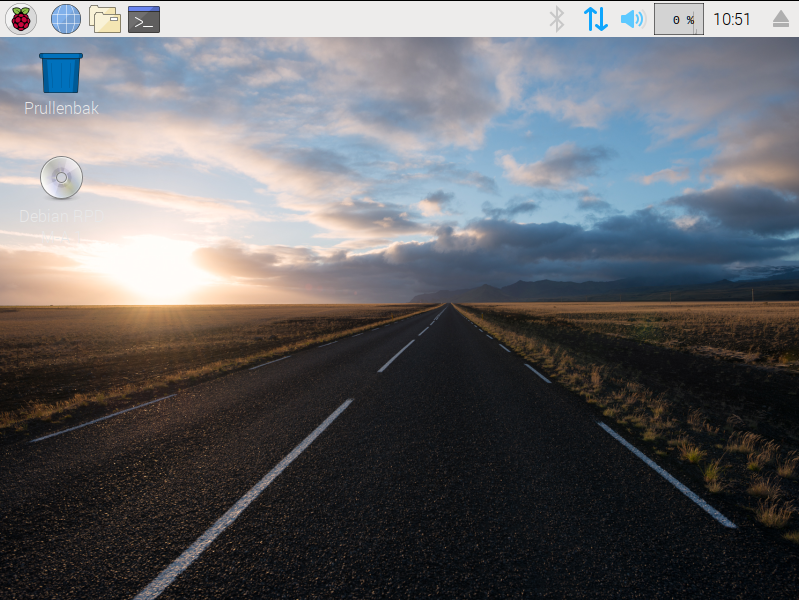
\includegraphics[scale=0.5]{raspbian.png}
    \caption{Raspbian desktopomgeving}
    \label{fig:raspbian}
\end{figure}
\begin{figure}[h]
    \centering
    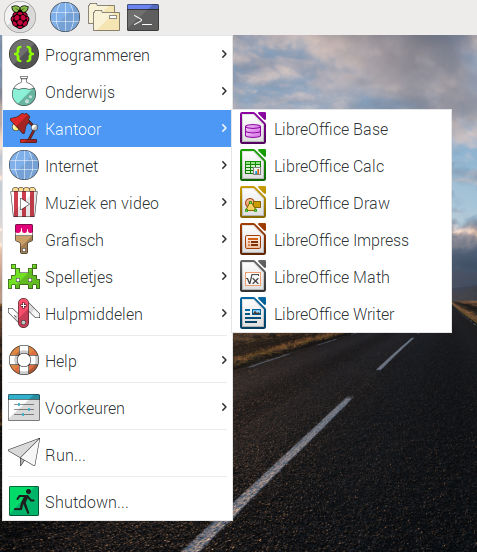
\includegraphics[scale=0.5]{raspbian-libreoffice.png}
    \caption{Raspbian heeft LibreOffice als kantoorsoftwarepakket}
    \label{fig:raspbian-libreoffice}
\end{figure}
Afhankelijk van het besturingssysteem dat draait op de Raspberry Pi 4, zijn een aantal software al
ge{\"i}nstalleerd.
Men kan er ook voor kiezen om een versie te installeren zonder deze voorge{\"i}nstalleerde software.
De Raspberry Pi Foundation ontwikkelt zelf een besturingssysteem voor de Raspberry Pi.
Dit besturingssysteem heet Raspbian en is gebaseerd op Debian.
In figuur \ref{fig:raspbian} is het bureaublad weergegeven van de versie van Raspbian met een
desktopomgeving.

Er is in dit paper ervoor gekozen om Raspbian te installeren met voorge{\"i}nstalleerde software.
Als men met de muis klikt op de framboos in de linkerbovenhoek, dan zal men verschillende software
aantreffen zoals te zien is in figuur \ref{fig:raspbian-libreoffice}.
Zo is bijvoorbeeld te zien dat Raspbian beschikt over LibreOffice.
Dit is tekstverwerkingssoftware vergelijkbaar met Microsoft Office.

Naast tekstverwerkingssoftware is er ook een browser.
Standaard in Raspbian is de Chromium Web Browser.
Ook bevat Raspbian een Terminal applicatie waarin men via commando's opdrachten kan uitvoeren.

\subsection{Mogelijkheden \& Toepassingen}
\begin{figure}[h]
    \centering
    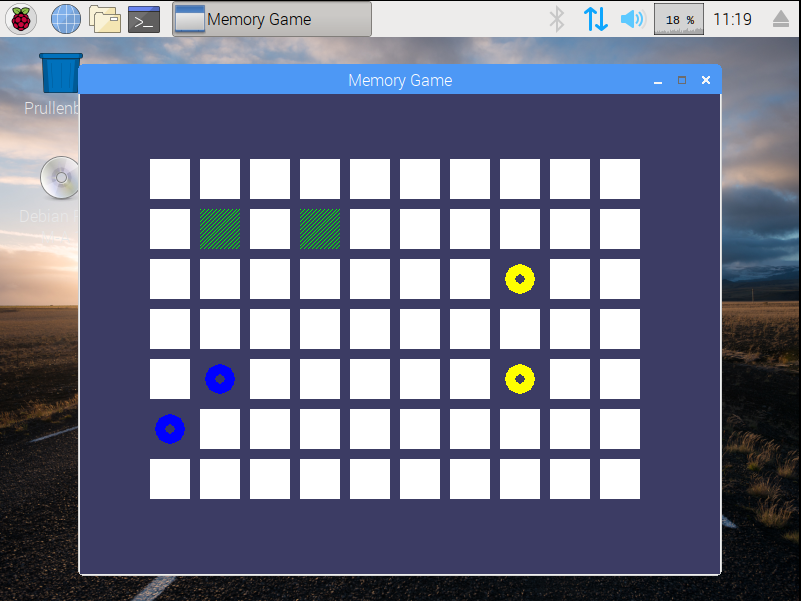
\includegraphics[scale=0.25]{raspbian-memory.png}
    \caption{Memory spel in Raspbian}
    \label{fig:raspbian-memory}
\end{figure}
Zoals al eerder gezegd is Raspberry Pi 4 een volledige computer.
Het enige verschil is dat hij in een formaat van een creditcard is.
Hij is dus erg compact en makkelijk te verwerken in allerlei projecten.
Met een Raspberry Pi 4 is het dus gewoon mogelijk om documenten te typen en om websites te bezoeken.

Echter heeft Raspberry Pi 4 ook flink een aantal nadelen.
Vanwege het ontbreken van een monitor, muis en toetsenbord, zal men deze apart moeten aanschaffen
als men de Raspberry Pi als desktop-computer wilt gebruiken.
Daarnaast is de kloksnelheid heel erg laag, namelijk 1.5 GHz.
Ook is het maximale beschikbare RAM geheugen heel erg weinig.

Ondanks deze beperkingen, zijn de mogelijkheden en toepassingen niet onaardig.
De simpele basistaken zoals tekstverwerking, internet en zeer lichte spelletjes spelen zijn gewoon
mogelijk.
Ter illustratie is in figuur \ref{fig:raspbian-memory} een simpele Memory spel te zien dat te spelen
is in Raspbian.

\section{Overeenkomsten en Verschillen}
In de vorige stukken zijn de eigenschappen, mogelijkheden en toepassingen van het Raspberry Pi- en
Arduino platform besproken.
In dit stuk zullen we de platformen vergelijken en de verschillen en overeenkomsten bespreken.
Deze bevindingen kunnen we dan vervolgens in de conclusie gebruiken om onze onderzoeksvraag te
beantwoorden.

\subsection{Architectuur \& Hardware}
Beide platformen zijn bedoeld voor gebruik in projecten waarin een computer nodig is, maar niet te
veel computer, dit is ook zichtbaar in het ontwerp van de hardware.
De afmeting van de Raspberry Pi 4 \cite{raspberry2019brief} zijn vergelijkbaar met verschillende
Arduino modellen, zoals de Arduino MEGA 2560 \cite{arduino2019mega} en de Arduino Uno
\cite{arduino2019uno}.
Daarnaast zijn er binnen beide platformen kleinere versies verkrijgbaar zoals de Raspberry Pi Zero
\cite{raspberry2019buy} en de Arduino Nano \cite{arduino2019products}.
Dit laat een belangrijke overeenkomst tussen de twee platformen zien, namelijk de focus op
compactheid.
Dit zorgt er voor dat de apparaten verwerkt kunnen worden in allerlei projecten, maar ook maakt het
de platformen toegankelijk voor niet-professionele toepassingen.
Denk aan hobbyisten die geen computer willen toewijden aan 1 taak, laat staan een serverkast gaan
opstellen.

De I/O van de Raspberry Pi, die bestaat uit USB, Micro HDMI en Ethernet \cite{raspberry20194bspecs},
is niet vergelijkbaar met bijvoorbeeld de Arduino Uno of MEGA 2560.
Bij Arduino's is de I/O vooral gebaseerd op digitale input/output pins
\cite{arduino2019mega,arduino2019uno}.
De I/O van de Raspberry Pi is wel vergelijkbaar met die van de Arduino Y{\'U}N, deze heeft als een
van de weinige Arduino's USB en Ethernet.
Deze Arduino is dan ook ontworpen om gebruikt te worden wanneer een internetverbinding nodig is
\cite{arduino2019yun}.
Dit laat een verschil zien in de doeleinden waarvoor de computers binnen de platformen ontworpen
zijn.
De Arduino is nuttig wanneer I/O op laag niveau nodig is, met volledige controle over elke bit van
in- en uitvoer.
De Raspberry Pi heeft de mogelijkheid om op een netwerk aangesloten te worden, en ook kan er
standaard USB-randapparatuur op aangesloten worden, dit maakt de Raspberry Pi nuttig voor projecten
waarbij I/O op hoger niveau nodig is.
Het verschil is ook niet vreemd wanneer rekening gehouden wordt met het feit dat de Raspberry Pi een
OS heeft om deze I/O aan te sturen, terwijl de Arduino dit niet heeft.

Arduino's zijn voorzien van een ATmega ARM microcontroller
\cite{arduino2019mega,arduino2019uno,arduino2019yun,arduino2019leonardo,kumar2015arduino} en de
Raspberry Pi 4 is voorzien van een quad-core Cortex-A72 ARMv8 processor \cite{raspberry2019brief}.
Beide platformen gebruiken dus een ARM processor.
ARM (Advanced RISC machine) processors zijn RISC processors en dit valt dus goed samen met de
filosofie van deze producten om de computer simpel te houden.
Een belangrijk verschil is wel dat de Arduino's een 8-bits singlecoreprocessor hebben terwijl de
Raspberry Pi 4 een 64-bits quad-core processor heeft \cite{raspberry2019brief}.
% opslag
% beeld

\subsection{Software}
De software is misschien wel het belangrijkste verschil tussen de twee platformen.
Zoals eerder gezegd zijn beide platformen nuttig voor gebruik in projecten, zowel voor hobbyisten
als professionele toepassingen.
Beide platformen zijn dan ook heel makkelijk te programmeren en nuttig als middel om te leren
programmeren \cite{raspberry2015what,jamieson2011arduino,rubio2013using}.
Toch is de manier hoe naar software gekeken wordt fundamenteel anders.
De Arduino heeft geen OS, de enige software die de Arduino uitvoert is dat wat de gebruiker op de
bootloader heeft gezet.
De Raspberry Pi heeft een OS.
De gebruiker kan zelf programma's schrijven en op het OS uitvoeren, of andere software gebruiken
uit de respository's van het OS.
Het gebruik van een Raspberry Pi lijkt dus veel op dat van een gewone computer.
De Arduino is niet interactief, de gebruiker zet zijn programma op de bootloader, en de Arduino
voert het uit.

\subsection{Mogelijkheden \& Toepassingen}
Als het gaat om automatisering en elektrische schakelingen, dan is de Arduino een betere keus.
Echter is de Raspberry Pi een volwaardige computer in tegenstelling tot de Arduino.
De Arduino kan binnenkomende gegevens van verschillende inputs verwerken en daarmee iets anders
aansturen via een output.
De Raspberry Pi lijkt meer op een volwaardige computer, maar dan sterk gereduceerd.
Een Raspberry Pi kan dingen doen als tekstverwerking, internetten via een browser of kleine games
draaien.
Zo heeft de Raspberry Pi veel meer aansluitingen voor randapparatuur en is de Arduino daar zeer
beperkt in.
Een voorbeeld is dat de Raspberry Pi standaard al voorzien is van een Ethernet aansluiting,
terwijl dit bij Arduino niet het geval is.

\subsection{Kosten}
De kosten voor een Raspberry Pi of de Arduino zijn zeer wisselend.
In beide gevallen hangt het er volledig van af welke generatie of versie men aanschaft.
Arduino verkoopt ontzettend veel verschillende printplaatjes die kunnen verschillen van ongeveer
\euro10 tot ongeveer \euro60 \cite{arduino2019arduino}.
De Raspberry Pi heeft een iets kleiner aanbod.
Hier zijn de prijzen ongeveer tussen \euro20--\euro60.
De uitzonderingen zijn de \emph{low budget} varianten: de Raspberry Pi Zero en de Raspberry Pi Zero W, die
respectievelijk \euro5 en \euro10 kosten \cite{kiwi2019zoeken}.
Uiteraard kan men er zoveel geld aan uitgeven als men wilt, aangezien er veel accessoires kunnen
worden toegevoegd aan zowel de Arduino als de Raspberry Pi.

\paragraph*{}
De overeenkomsten en verschillen zijn nu benoemd en uitgelegd, deze zullen worden gebruikt in het
volgende hoofdstuk, dat zal de conclusie zijn.

\section{Conclusie}
De onderzoeksvraag luidt: `Wat zijn de verschillen tussen Raspberry Pi en Arduino en welke is
beter?'
Nu de resultaten bekend zijn, kan deze onderzoeksvraag beantwoord worden.

De twee mini-computers verschillen veel van elkaar.
Het is daarom lastig te zeggen welke van de twee het beste is.
Het grootste verschil zit in het besturingssysteem en in de processor.
De Raspberry Pi gebruikt een besturingssysteem en heeft een 64-bits quad-core processor, terwijl de
Arduino geen besturingssysteem heeft en een 8-bits singlecoreprocessor.
Dit is het grootste noemenswaardige verschil en dit leidt tot de conclusie dat de Raspberry Pi beter
gebruikt kan worden voor grotere, zwaardere projecten, terwijl de Arduino het best gebruikt kan
worden voor wat lichtere en kleine projecten.

Het resultaat van dit kan van belang zijn voor de producenten van de Arduino en Raspberry Pi.
Dit is in de eerste plaats, omdat zij kunnen zien waar zij beter presteren dan hun concurrent, en
dus tegelijk ook waar zij minder goed presteren dan hun concurrent.
Als zij het van belang vinden om in elk opzicht beter te zijn, dan kunnen zij dit onderzoek
gebruiken om hun product beter te maken.
Dit onderzoek kan ook van belang zijn om te kijken of zij zich richten op de goede doelgroep, of dat
zij zich moeten richten op een ander doelgroep.
Stel dat de producent ziet dat de Arduino beter verkoopt dan de Raspberry Pi, terwijl de Raspberry
Pi betere specificaties heeft, dan kan de producent van de Raspberry Pi zich focussen om meer
reclame te maken, en hoeft zij zich niet bezig te houden met productontwikkeling, maar kan de focus
meer liggen op marketing bijvoorbeeld.

Dit onderzoek kan ook van waarde zijn voor de consument.
Als een consument graag een groot project zou willen draaien op een mini-computer, dan kan beter een
Raspberry Pi gebruikt worden.
Als de consument een klein project of enkele opdrachten prefereert, dan kan beter een Arduino
gebruikt worden.
Dit onderzoek kan de consument helpen om een keuze te maken tussen de Arduino en de Raspberry Pi.
Een Arduino wordt vooral gebruikt voor geautomatiseerde taken en elektrische schakelingen, terwijl
een Raspberry Pi gebruikt wordt voor taken die een volwaardige desktop-pc zou kunnen uitvoeren.

In dit paper is een antwoord gevonden op de onderzoeksvraag.
Dit is vooral theoretisch gedaan met een paar voorbeelden uit de praktijk.
Dit onderzoek kan nog een keer gedaan worden, met dezelfde onderzoeksvraag, maar dan met veel
praktijkgericht onderzoek, dus bijvoorbeeld verschillende soorten opdrachten uit voeren met beide
mini-computers, waardoor er getest kan worden welke beter functioneert voor specifieke opdrachten.

\printbibliography

\section{Logboek}
\begin{tabular}{ll}
    \textbf{Wat}                  & \textbf{Wie}   \\
    \hline
    Samenvatting                  & Wilmar         \\
    Inleiding                     & Wilmar         \\
    Arduino                       & Jacob-Jan      \\
    Arduino Uitgewerkt Voorbeeld  & Kenneth        \\
    Raspberry Pi                  & Kenneth        \\
    Overeenkomsten \& Verschillen & Luuk \& Herman \\
    Conclusie                     & Wilmar         \\
    \hline
    Opmaak \& Lay-out             & Luuk           \\
    Editing                       & Luuk
\end{tabular}
\end{document}
